%%%%%%%%%%%%%%%%%%%%%%%%%%%%%%%%%%%%%%%%%%%%%%%%%%%%%%%%%%%%%%%%%%%%%%
% Problem statement
\begin{statement}[
  problempoints=50,
  timelimit=1 sekunda,
  memorylimit=512 MiB,
]{Pod starim krovovima}

\setlength\intextsep{-0.1cm}
\begin{wrapfigure}[7]{r}{0.16\textwidth}
\centering
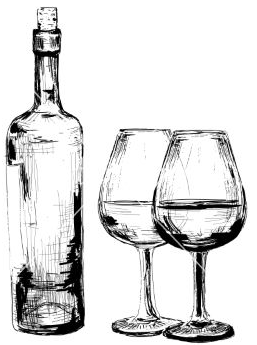
\includegraphics[width=0.16\textwidth]{img/psk.png}
\end{wrapfigure}

\textbf{Mjesto radnje:} legendarna starozagrebačka gostionica \textit{Kod
Žnidaršića}.

\textbf{Vrijeme radnje:} početak druge polovice tridesetih godina dvadesetog
stoljeća.

\textbf{Radnja:} Franjo za šankom s prijateljima razgovara o stanju u
Abesiniji. Njegov sin, mali Perica, sjedi u kutu za stolom. Na stolu ispred
Perice stoji $N$ čaša označenih brojevima od $1$ do $N$. Za svaku čašu znamo
koliko u njoj trenutno ima tekućine i kolika je njena zapremnina u nanolitrima.
Zapremnina je najveća količina tekućine koju možemo uliti u čašu.

\textbf{Problem:} Malog Pericu zanima koliko najviše čaša može isprazniti
prelijevanjem tekućine između čaša. Pod prelijevanjem tekućine iz jedne u
drugu čašu podrazumijevamo postupak kojim svu ili neki cjelobrojni dio (u
nanolitrima) tekućine iz jedne čaše prelijemo u drugu čašu. Prilikom
prelijevanja tekućina se ne smije proliti po stolu.

Ispišite traženi broj ispražnjenih čaša te dodatno ispišite količinu tekućine u
svakoj čaši u trenutku kada je ispražnjeno najviše čaša što se moglo.  Ako
ima više mogućnosti, ispišite bilo koju. Primijetite da nije potrebno
minimizirati broj prelijevanja.

%%%%%%%%%%%%%%%%%%%%%%%%%%%%%%%%%%%%%%%%%%%%%%%%%%%%%%%%%%%%%%%%%%%%%%
% Input
\subsection*{Ulazni podaci}
U prvom je retku prirodan broj $N$ $(1 \le N \le 1\ 000)$ iz teksta zadatka.

U sljedećih $N$ redaka su po dva broja, cijeli broj $T_i$ $(0 \le T_i \le 10^9)$
i prirodan broj $Z_i$ $(1 \le Z_i \le 10^9)$ koji predstavljaju trenutnu
količinu tekućine te zapremninu čaše s oznakom $i$. Obje su vrijednosti dane
u nanolitrima te trenutna količina tekućine u čaši ne može premašiti njenu
zapremninu, odnosno vrijedi $T_i \le Z_i$.

%%%%%%%%%%%%%%%%%%%%%%%%%%%%%%%%%%%%%%%%%%%%%%%%%%%%%%%%%%%%%%%%%%%%%%
% Output
\subsection*{Izlazni podaci}
U prvi redak ispišite najveći broj čaša koji možemo isprazniti.

U drugi redak ispišite traženu količinu tekućine (u nanolitrima) u čašama
počevši od one s oznakom $1$ pa sve do one s oznakom $N$.

%%%%%%%%%%%%%%%%%%%%%%%%%%%%%%%%%%%%%%%%%%%%%%%%%%%%%%%%%%%%%%%%%%%%%%
% Scoring
\subsection*{Bodovanje}
Točan ispis prvog retka vrijedi $4$ boda, a točan ispis drugog retka vrijedi $1$
bod za svaki testni primjer.

U testnim primjerima vrijednima $20$ bodova sve će čaše biti iste
zapremnine.

%%%%%%%%%%%%%%%%%%%%%%%%%%%%%%%%%%%%%%%%%%%%%%%%%%%%%%%%%%%%%%%%%%%%%%
% Examples
\subsection*{Probni primjeri}
\begin{tabularx}{\textwidth}{X'X'X}
\sampleinputs{test/psk.dummy.in.1}{test/psk.dummy.out.1} &
\sampleinputs{test/psk.dummy.in.2}{test/psk.dummy.out.2} &
\sampleinputs{test/psk.dummy.in.3}{test/psk.dummy.out.3}
\end{tabularx}

\textbf{Pojašnjenje drugog probnog primjera:}
Jedan od mogućih postupaka prelijevanja je
\begin{enumerate}
  \item sve iz čaše $1$ u čašu $2$.
  \item sve iz čaše $2$ u čašu $4$.
  \item četiri nanolitra iz čaše $3$ u čašu $4$
  \item jedan nanolitar iz čaše $3$ u čašu $5$.
\end{enumerate}
Sada su čaše s oznakama $1$, $2$ i $3$ u potpunosti prazne.

%%%%%%%%%%%%%%%%%%%%%%%%%%%%%%%%%%%%%%%%%%%%%%%%%%%%%%%%%%%%%%%%%%%%%%
% We're done
\end{statement}

%%% Local Variables:
%%% mode: latex
%%% mode: flyspell
%%% ispell-local-dictionary: "croatian"
%%% TeX-master: "../hio.tex"
%%% End:
